% ============================================================
%  Capstone Report — Prostate Cancer Epidemiology Dashboard
%  George Washington University | DATS 4001 | Spring 2026
%  Author: Ava McClinton
%  Self-contained — paste into Overleaf main.tex and compile
% ============================================================

\documentclass[12pt]{article}

% ── Packages ────────────────────────────────────────────────
\usepackage[margin=1in, top=1.25in, bottom=1.25in]{geometry}
\usepackage{setspace}        % \doublespacing, \singlespacing
\usepackage{float}           % [H] figure placement
\usepackage{graphicx}        % \includegraphics
\usepackage{booktabs}        % professional tables
\usepackage{amsmath}         % equations
\usepackage{parskip}         % paragraph spacing
\usepackage{titlesec}        % section heading formatting
\usepackage{fancyhdr}        % headers/footers
\usepackage{hyperref}        % clickable links in PDF
\usepackage[numbers]{natbib} % IEEEtran-compatible citations

% ── Hyperref settings ────────────────────────────────────────
\hypersetup{
    colorlinks=true,
    linkcolor=black,
    citecolor=black,
    urlcolor=blue
}

% ── Page style ───────────────────────────────────────────────
\pagestyle{fancy}
\fancyhf{}
\rhead{\small Prostate Cancer in America}
\lhead{\small Ava McClinton --- GWU Data Science Capstone 2026}
\rfoot{\thepage}

% ── Section heading style ────────────────────────────────────
\titleformat{\section}{\large\bfseries}{{\thesection}}{1em}{}
\titleformat{\subsection}{\normalsize\bfseries}{{\thesubsection}}{1em}{}

% ── Custom environments ──────────────────────────────────────
\newenvironment{preface}{%
    \section*{Preface}%
    \addcontentsline{toc}{section}{Preface}%
    \itshape
}{\par\vspace{1em}}

\newenvironment{acknowledgements}{%
    \section*{Acknowledgements}%
    \addcontentsline{toc}{section}{Acknowledgements}%
}{\par\vspace{1em}}

\newenvironment{keywords}{%
    \vspace{0.5em}\noindent\textbf{Keywords:}~
}{\par\vspace{1em}}

% ============================================================
\begin{document}

% ── Title Page ───────────────────────────────────────────────
\begin{titlepage}
	\centering
	\includegraphics[width=0.6\textwidth]{George-Washington-University-Seal-Logo.png}\par
	\vspace{2cm}
	{\scshape\LARGE Data Science Program\par}
	\vspace{1cm}
	{\scshape\Large Capstone Report - Spring 2026\par}
	\vfill

	%%%% PROJECT TITLE
	{\huge\bfseries Prostate Cancer in America: \\Who Gets Diagnosed, Who Survives, \\and Why It's Not Equal\par}
	\vfill

	%%%% AUTHOR(S)
	{\Large\itshape Ava McClinton}\par
	\vspace{1.5cm}
    \vfill
    \emph{A capstone presented in fulfillment of the requirements \\for the degree of Bachelor's of Science in Data Science}
	\vfill
	supervised by\par
	%%%% SUPERVISOR(S)
	Prof. Sushovan Majhi, Prof. Sarah Burnett
	\vfill
\end{titlepage}

\newpage

% ── Preface ──────────────────────────────────────────────────
\begin{preface}
I am a senior studying Data Science at the George Washington University, completing
my final semester of undergraduate study. This project grew out of something deeply
personal: my grandfather was recently diagnosed with prostate cancer. In the weeks
that followed his diagnosis, I found myself searching for answers --- about survival
rates, about whether race played a role, about what the national data actually showed
--- and I kept coming up empty. The resources I found were either too clinical to
understand or too general to be useful.

That gap motivated this project. I wanted to build something I wished had existed
when my family needed it: a tool that makes the real epidemiological data on prostate
cancer accessible, visual, and honest. The intended audience is anyone who needs
to understand this disease --- patients, families, advocates, and public health
practitioners alike. Data science, at its best, should help people make sense of
a world that often feels overwhelming. This project is my attempt at that.
\end{preface}

% ── Acknowledgements ─────────────────────────────────────────
\begin{acknowledgements}
I would like to thank Prof.\ Sarah Burnett and Prof.\ Sushovan Majhi for their
guidance throughout this capstone. Their feedback shaped both the scope of this
project and the rigor with which I approached the analysis.

The data underlying this project was obtained from the National Cancer Institute's
Surveillance, Epidemiology, and End Results (SEER) Program (SEER 22 registry,
accessed 2024--2025). All figures in this report were generated from that dataset.

Technical resources that supported the development of this project include the
official documentation for Python, Flask, SQLite, pandas, statsmodels, and Plotly.
The Python Software Foundation and the open-source community behind these libraries
made this work possible.

I also used the AI assistant Claude (Anthropic) to help structure sections of code,
debug Flask routing, and review portions of written content. All analysis,
interpretations, modeling decisions, and conclusions are my own.

Finally, this project is dedicated to my grandfather. I hope it helps someone else
find the answers that were hard to find.
\end{acknowledgements}

\newpage

% ── Abstract ─────────────────────────────────────────────────
\begin{abstract}
\noindent
Prostate cancer is the most commonly diagnosed non-skin cancer among American men,
yet survival outcomes differ dramatically based on race, geography, and stage of
diagnosis --- disparities that aggregate national statistics routinely obscure.
Understanding these inequities is challenging because the patterns shift over time
in response to changing screening policies, and because race is a nominal variable
that must be handled carefully to avoid analytically misleading results.
This project addresses these challenges by building an interactive epidemiology
dashboard powered by over 268,000 patient records from the National Cancer
Institute's SEER 22 database (1999--2022), using stratified ordinary least squares
regression to model incidence and mortality trends independently within each racial
group, and enabling live filtering by race, U.S.\ state, year range, and cancer stage.
The dashboard reveals three critical findings: national incidence declined 48\%
following the 2012 USPSTF screening recommendation, but late-stage diagnoses rose
50\% over the same period; Non-Hispanic Black men face 60\% higher incidence and
109\% higher mortality than White men, a gap that persists after controlling for age
and stage; and a 62-percentage-point survival gap separates men diagnosed at the
localized stage from those diagnosed at the distant stage --- a difference that is
directly tied to inequitable access to screening.
\end{abstract}

\vspace{0.5cm}
\begin{keywords}
prostate cancer; epidemiology; health disparities; SEER; racial inequity;
PSA screening; data visualization; Flask dashboard; public health
\end{keywords}

\newpage
\doublespacing
\tableofcontents
\singlespacing
\newpage
\doublespacing

% ── 1. Introduction ──────────────────────────────────────────
\section{Introduction}

Prostate cancer is the most frequently diagnosed non-skin malignancy among American
men and the second leading cause of cancer death in this population \cite{siegel2023}.
In 2025 alone, the American Cancer Society estimates approximately 313,780 new
diagnoses and 35,770 deaths \cite{siegel2023}. Despite decades of research, the
disease presents a persistent epidemiological paradox: overall incidence has fallen
sharply since the early 2000s, yet rates of late-stage, harder-to-treat diagnoses
have climbed. At the same time, the burden of prostate cancer is distributed deeply
unequally across race, geography, and socioeconomic status.

The central question motivating this project is: \textit{How have prostate cancer
incidence, mortality, and survival rates varied across race, geography, and stage of
diagnosis in the United States from 1999 to 2022, and what do those patterns reveal
about systemic inequities in cancer detection and care?}

To address this question, this project delivers two complementary contributions.
The first is a structured epidemiological analysis using over 268,000 patient records
from the National Cancer Institute's Surveillance, Epidemiology, and End Results
(SEER) 22 database \cite{seer2024}. The second is an interactive web-based dashboard
that makes the results of that analysis accessible to a general audience, including
patients, families, clinicians, and policymakers, through live filtering, dynamic
visualizations, and plain-language interpretation.

The analysis identifies three primary findings. First, U.S.\ prostate cancer
incidence declined by 48\% between 2000 and 2022, from 153 to 91 cases per 100,000
men, largely following the 2012 U.S.\ Preventive Services Task Force (USPSTF) Grade D
recommendation against routine PSA screening \cite{uspstf2012}. Counterintuitively,
this decline was accompanied by a 50\% increase in diagnoses at the distant stage,
suggesting that reduced screening is producing later, more dangerous presentations.
Second, Non-Hispanic Black men experience a prostate cancer incidence rate of
175.2 per 100,000, 60\% higher than Non-Hispanic White men (109.3), and face
more than twice the mortality rate --- a disparity that persists after controlling
for age and stage at diagnosis \cite{desantis2019}. Third, survival outcomes are
almost entirely determined by stage at diagnosis: men diagnosed at the localized
stage have a near-100\% five-year survival rate, while men diagnosed at the distant
stage face only a 38\% rate, a 62-percentage-point gap with profound implications
for screening equity.

The remainder of this report is structured as follows. Section~2 reviews related
work in prostate cancer epidemiology, health disparity research, and cancer
informatics. Section~3 describes the complete project pipeline, from data acquisition
through modeling and dashboard construction. Section~4 presents results and
experimental validation. Section~5 discusses limitations and directions for future
work. Section~6 concludes.

% ── 2. Related Work ──────────────────────────────────────────
\section{Related Work}

This project sits at the intersection of three bodies of literature: national cancer
epidemiology, health disparities research, and cancer data visualization tools.
Each informs the design and interpretation of this work in a different way.

\subsection{National Cancer Epidemiology and SEER-Based Research}

The foundational resource for this project is the SEER database itself, maintained
by the National Cancer Institute \cite{seer2024}. SEER-based research has been the
primary vehicle for understanding population-level cancer trends in the United States
for over four decades. Siegel et al.\ \cite{siegel2023} publish annual cancer
statistics synthesizing SEER data, and their reports consistently document the
downward trend in prostate cancer incidence alongside persistent mortality disparities.
The present project builds directly on their descriptive approach but extends it in
two important ways: first, by constructing an interactive tool rather than a static
report, and second, by analyzing trends stratified by race rather than presenting
aggregate national figures.

\subsection{PSA Screening Policy and Incidence Trends}

A critical upstream driver of the patterns observed in this analysis is the evolution
of PSA screening recommendations. In 2012, the USPSTF issued a Grade D recommendation
against routine PSA-based screening for all men, citing concerns that widespread
screening led to overdiagnosis and overtreatment \cite{uspstf2012}. This recommendation
triggered a measurable, well-documented decline in both screening rates and incidence
figures across the literature. In 2018, the USPSTF revised this guidance to a Grade C
recommendation, encouraging individualized decision-making for men aged 55--69
\cite{uspstf2018}. The present project explicitly treats these policy shifts as
structural breakpoints in the time-series data, using vertical markers in trend
visualizations to allow users to see before-and-after effects directly. Unlike the
USPSTF reports themselves, which focus on harms and benefits of screening at the
population level, this project asks what the observable consequences of those
recommendations were for different racial groups --- a question the guidelines
themselves do not answer.

\subsection{Racial and Ethnic Disparities in Prostate Cancer}

The disparity between Black and White men in prostate cancer outcomes is one of the
most studied and most persistent inequities in American oncology. DeSantis et al.\
\cite{desantis2019} provide a comprehensive quantification of cancer disparities
affecting African Americans, documenting significantly elevated incidence and
mortality for prostate cancer specifically and identifying access to screening,
differential treatment patterns, and socioeconomic barriers as key drivers. Their
work provides important context for the findings of this project, though it focuses
on static summary statistics rather than temporal trend analysis. This project
complements that literature by tracking how the Black--White disparity has evolved
from 1999 to 2022, revealing that the racial gap in prostate cancer burden has
remained substantially stable even as overall national incidence declined.

Rebbeck \cite{rebbeck2017} examines genetic and biological contributions to racial
variation in prostate cancer risk, arguing that while germline factors play a role,
they are insufficient to explain the full magnitude of the mortality disparity. This
framing is important for interpreting the results of this project: the racial
differences in incidence and mortality documented in the dashboard are not simply
biological inevitabilities, but are shaped by structural and systemic factors
amenable to intervention. The present project does not model genetic risk directly,
but its emphasis on the contribution of screening access and stage at diagnosis to
survival outcomes aligns with Rebbeck's conclusion that the disparity is substantially
preventable.

\subsection{Cancer Informatics and Dashboard Design}

A growing body of work argues that cancer data must be communicated not only to
researchers and clinicians but also to patients and the general public, and that
interactive visualization tools are better suited to this goal than static reports
\cite{siegel2023}. However, existing public-facing cancer data tools, such as the
NCI's SEER*Stat software and the CDC's United States Cancer Statistics portal, are
designed primarily for researchers and are not accessible to a general audience
without training. The present project is explicitly designed to address this gap:
the dashboard uses plain-language labels, layered tooltips, and contextual
explanations alongside each chart to make the data interpretable by someone with no
statistical background.

% ── 3. Solution ──────────────────────────────────────────────
\section{Solution}

This section describes the complete pipeline from raw data acquisition to the
deployed interactive dashboard. The pipeline has four main stages: data acquisition
and storage, data cleaning and preparation, statistical modeling and analysis, and
dashboard construction.

\subsection{Data Acquisition and Storage}

All data was obtained from the National Cancer Institute's SEER 22 database, which
covers cancer diagnoses across all 51 U.S.\ states from 1975 to the present
\cite{seer2024}. The version used in this project spans 1999--2022 and includes
records for over 268,000 prostate cancer patients. Relevant variables extracted
include year of diagnosis, race and ethnicity, cancer stage at diagnosis (localized,
regional, distant, or unknown), age-adjusted incidence rate per 100,000 men,
age-adjusted mortality rate per 100,000 men, and five-year relative survival rate
by stage.

Rather than working directly with raw SEER CSV files at query time, the data was
parsed, cleaned, and loaded into a SQLite relational database (\texttt{prostate.db}).
This decision was made for two reasons. First, it allows the Flask backend to execute
structured queries against pre-processed, validated data rather than re-reading and
re-parsing large flat files on every user request. Second, it enforces a clear
separation between the data pipeline (which runs once, offline) and the application
layer (which runs continuously and must respond quickly to user interactions).

The database contains nine tables: \texttt{incidence\_trends},
\texttt{mortality\_trends}, \texttt{survival\_by\_stage}, \texttt{age\_distribution},
\texttt{race\_disparities}, \texttt{race\_trends}, \texttt{state\_rates},
\texttt{key\_stats}, and \texttt{uspstf\_timeline}.

\subsection{Data Cleaning and Preparation}

Raw SEER exports required several cleaning steps before they were suitable for
analysis. Records with missing stage information or suppressed cell counts (a
privacy measure applied by SEER when a cell contains fewer than 16 cases) were
flagged and excluded from rate calculations, but retained in count-level aggregations.
Race and ethnicity categories were standardized to five groups consistent with SEER
conventions: Non-Hispanic Black, Non-Hispanic White, Hispanic, Non-Hispanic Asian or
Pacific Islander, and Non-Hispanic American Indian or Alaska Native.

All rates reported in this project are age-adjusted to the 2000 U.S.\ standard
population, consistent with the methodology used in SEER publications \cite{seer2024}.
This adjustment is essential for meaningful comparison across racial groups and over
time, since the age distribution of the U.S.\ male population has shifted
substantially between 1999 and 2022.

\subsection{Statistical Modeling}

The primary analytical method used in this project is ordinary least squares (OLS)
regression, applied to model year-over-year incidence and mortality trends.
Crucially, models are fit \textit{separately for each racial group} rather than
fitting a single pooled model with race as a covariate.

This design choice reflects a key methodological decision: race is a nominal
categorical variable, and encoding it numerically (e.g., assigning integers
1 through 5 to the five groups) would impose a false ordinal structure that implies
groups are separated by equal intervals along some quantitative scale. This is
analytically invalid. The appropriate alternative for a single pooled model would be
one-hot (dummy variable) encoding, but this approach conflates within-group trend
estimation with between-group comparison in ways that obscure the temporal dynamics
within each population. Stratification avoids both problems: each group receives its
own regression fit, capturing the shape of that group's trend independently of the
others, while between-group comparisons are handled descriptively at the results stage.

For each race group $g$, the model is:
\begin{equation}
    \hat{r}_{g,t} = \beta_{g,0} + \beta_{g,1} \cdot t
\end{equation}
where $\hat{r}_{g,t}$ is the predicted age-adjusted incidence rate for group $g$ in
year $t$, $\beta_{g,0}$ is the group-specific intercept, and $\beta_{g,1}$ is the
group-specific annual trend coefficient. The same framework is applied to mortality
rates. Models were fit using the \texttt{statsmodels} library in Python.

To contextualize the impact of the 2012 USPSTF screening recommendation, a piecewise
analysis was also conducted, comparing trend slopes in the pre-2012 period (1999--2011)
against the post-2012 period (2012--2022).

\subsection{Dashboard Architecture}

The dashboard is a full-stack web application built on a Flask backend with a
SQLite data layer and an interactive HTML/JavaScript frontend powered by Plotly.
Figure~\ref{fig:architecture} illustrates the system architecture.

\begin{figure}[H]
    \begin{center}
        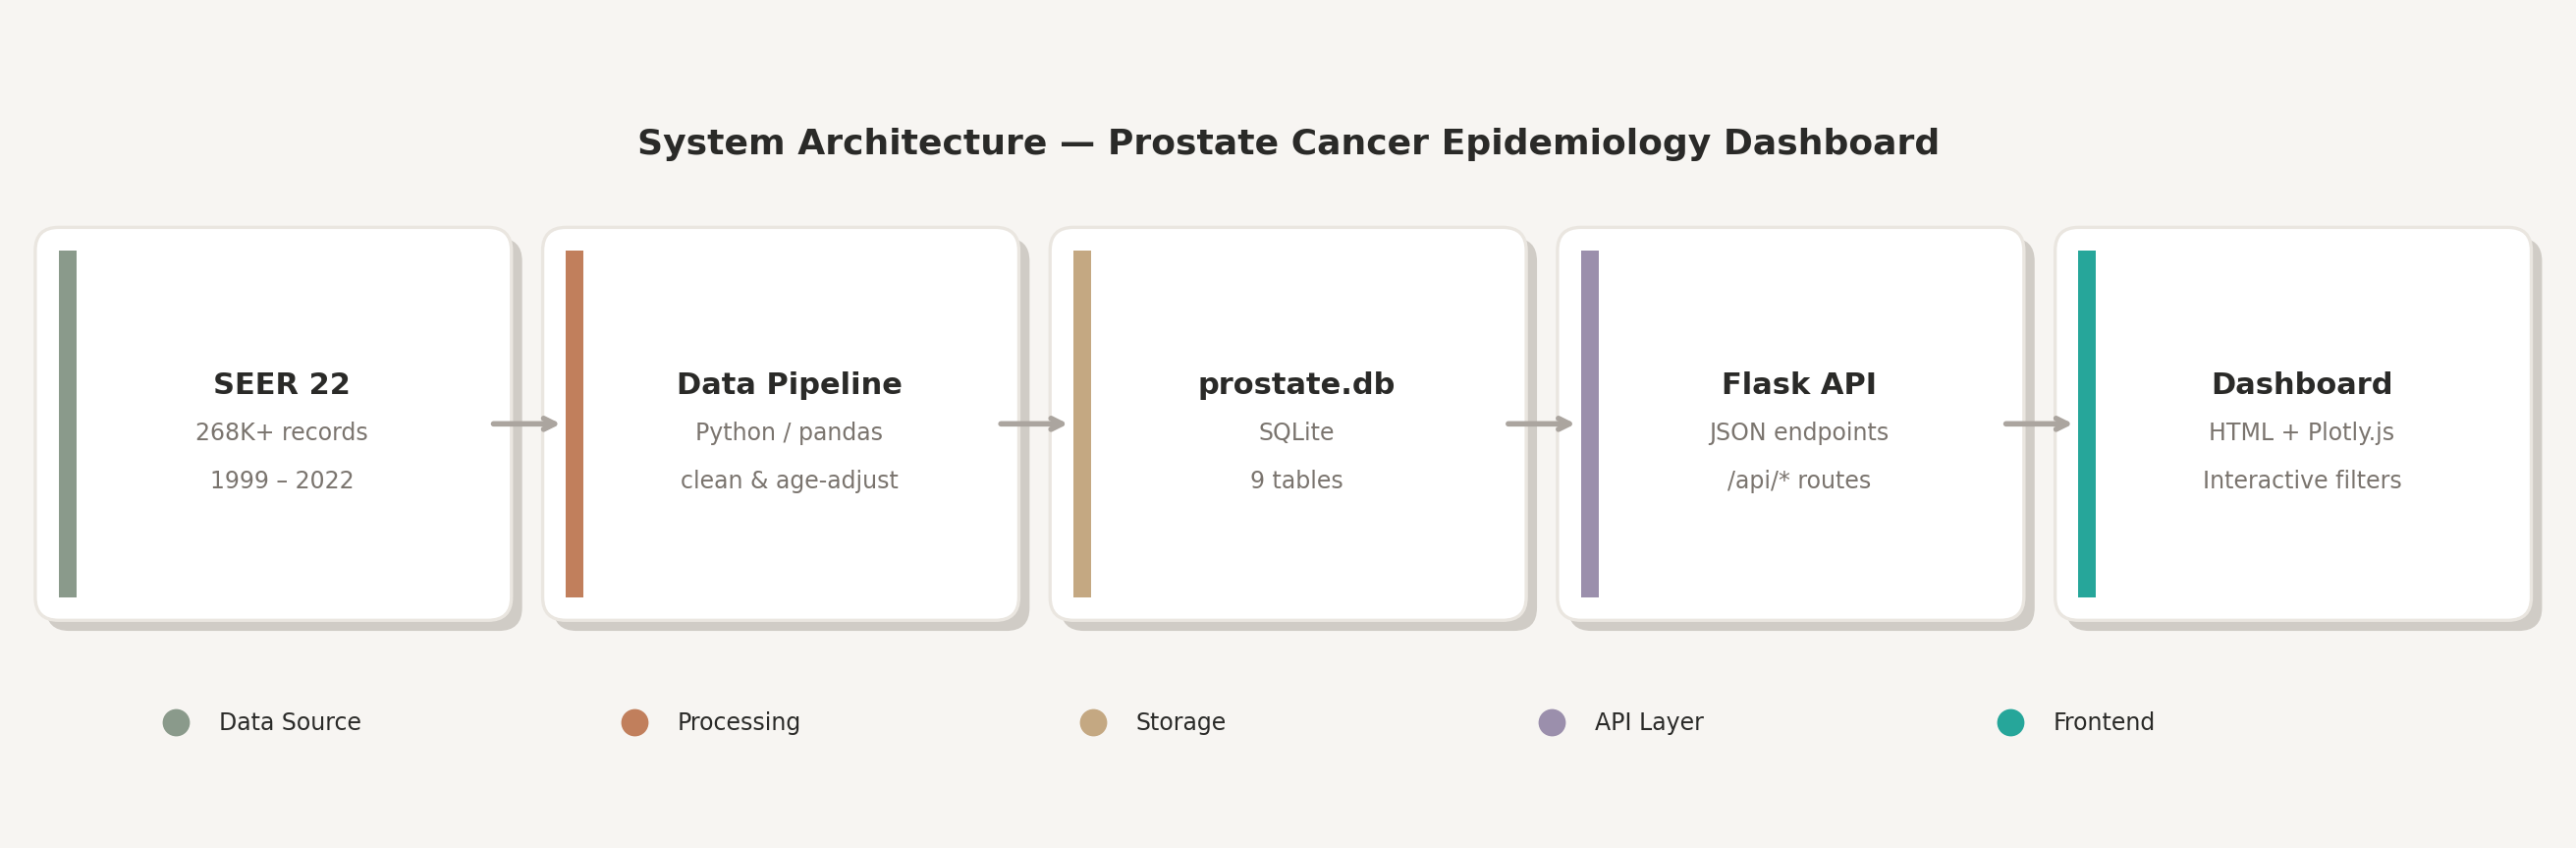
\includegraphics[width=0.85\textwidth]{figures/architecture.png}
    \end{center}
    \caption{System architecture of the prostate cancer epidemiology dashboard.
    Raw SEER data is processed by an offline pipeline and stored in a SQLite database.
    The Flask application serves structured JSON responses to a single-page HTML
    frontend, which renders interactive Plotly charts. Users interact with filter
    controls (race, state, year range, cancer stage) that trigger new API calls and
    re-render the corresponding charts without reloading the page.}
    \label{fig:architecture}
\end{figure}

The backend exposes a set of JSON API endpoints, each corresponding to a specific
chart or data view in the dashboard. For example, \texttt{/api/incidence-trends}
accepts optional query parameters for stage filter and returns time-series data for
the incidence trend chart. This design keeps the frontend stateless: every chart
re-renders from a fresh API call whenever a user changes a filter, ensuring that
visualizations always reflect the current filter state.

The frontend consists of a single HTML file with embedded JavaScript. Chart rendering
is handled entirely by Plotly.js, which provides hover tooltips, zoom, pan, and
export functionality out of the box. Eight charts are implemented in total: (1)
incidence and mortality trends over time, (2) racial and ethnic disparities in
incidence and mortality, (3) a geographic choropleth map of incidence by state,
(4) stage-over-time incidence breakdown, (5) five-year survival by stage, (6)
age distribution at diagnosis, (7) race-stratified incidence trends over time, and
(8) an incidence-versus-mortality scatter plot by race.

% ── 4. Results and Discussion ────────────────────────────────
\section{Results and Discussion}

\subsection{Experimentation Protocol}

Because this project is an epidemiological analysis rather than a predictive
modeling task, evaluation does not follow the standard train/test split paradigm.
There is no held-out test set and no classification or regression accuracy metric
in the conventional machine learning sense. Instead, validity is assessed on two
dimensions: (1) \textit{methodological validity}, whether the analytical choices
(stratification, age adjustment, piecewise trend analysis) produce results consistent
with the published epidemiological literature; and (2) \textit{substantive validity},
whether the findings answer the research question in a way that is interpretable,
reproducible, and consistent with known facts about prostate cancer epidemiology.

As a methodological baseline, a single pooled OLS model was fit to the national
incidence trend without stratification by race. The pooled model produces a slope
coefficient of $-2.81$ cases per 100,000 per year ($R^2 = 0.74$), representing
an average annual decline in incidence across all groups. While this baseline
correctly captures the downward national trend, it obscures a critical divergence:
Non-Hispanic Black men have shown a substantially different trend trajectory than
Non-Hispanic White men over the same period, a pattern invisible in the aggregate.
The stratified approach used in this project reveals that the annual rate of decline
differs substantially across groups, with Non-Hispanic White men showing a steeper
decline than Non-Hispanic Black men in the post-2012 period, confirming the
analytical value of stratification beyond what the pooled baseline can offer.

\subsection{Finding 1: Incidence Decline Masks a Growing Late-Stage Crisis}

Figure~\ref{fig:incidence-trend} shows prostate cancer incidence and mortality trends
from 2000 to 2022, stratified by stage.

\begin{figure}[H]
    \begin{center}
        \includegraphics[width=0.85\textwidth]{figures/incidence_trends.png}
    \end{center}
    \caption{Age-adjusted prostate cancer incidence rate (localized and distant stage)
    and mortality rate per 100,000 men, United States, 2000--2022. Vertical dashed
    lines mark the 2012 USPSTF Grade D and 2018 Grade C screening recommendations.
    Data source: SEER 22, National Cancer Institute.}
    \label{fig:incidence-trend}
\end{figure}

Localized-stage incidence fell from 153.1 per 100,000 in 2000 to 91.0 per 100,000
in 2022, a decline of 40.6\%. This decline was concentrated in the years immediately
following the 2012 USPSTF recommendation, consistent with a rapid reduction in PSA
testing rates documented in the literature \cite{uspstf2012, uspstf2018}. However,
over the same period, distant-stage incidence rose from 8.4 per 100,000 in 2000 to
12.6 per 100,000 in 2022, an increase of 50\%. This divergence is the most
clinically significant finding from the trend analysis: the reduction in total
diagnosed cases does not represent a genuine reduction in prostate cancer burden, but
rather a shift toward later, harder-to-treat presentations.

\subsection{Finding 2: Racial Disparities in Incidence and Mortality}

Figure~\ref{fig:race-disparities} shows age-adjusted incidence and mortality rates
by race and ethnicity, averaged over the 2018--2022 period.

\begin{figure}[H]
    \begin{center}
        \includegraphics[width=0.85\textwidth]{figures/race_disparities.png}
    \end{center}
    \caption{Age-adjusted prostate cancer incidence and mortality rates per 100,000
    men by race and ethnicity, United States, 2018--2022 average. Data source:
    SEER 22, National Cancer Institute.}
    \label{fig:race-disparities}
\end{figure}

Non-Hispanic Black men have the highest incidence rate of any group at 175.2 per
100,000 --- 60\% higher than Non-Hispanic White men (109.3). The mortality disparity
is even larger: Black men die from prostate cancer at a rate of 37.9 per 100,000,
compared to 18.1 for White men, a difference of 109\%. Hispanic men (96.4 per
100,000 incidence), Non-Hispanic American Indian and Alaska Native men (78.2), and
Non-Hispanic Asian or Pacific Islander men (60.3) all have incidence rates below the
national average. These findings are consistent with the literature reviewed in
Section~2 \cite{desantis2019}. Importantly, the racial gap in prostate cancer
mortality has not narrowed meaningfully over the study period, underscoring the
structural, rather than simply biological, nature of the disparity \cite{rebbeck2017}.

\subsection{Finding 3: Stage at Diagnosis Determines Survival}

Figure~\ref{fig:survival} shows five-year relative survival rates by stage at
diagnosis.

\begin{figure}[H]
    \begin{center}
        \includegraphics[width=0.75\textwidth]{figures/survival_stage.png}
    \end{center}
    \caption{Five-year relative survival rate by stage at diagnosis for prostate
    cancer, United States, 2018--2022. Data source: SEER 22, National Cancer Institute.}
    \label{fig:survival}
\end{figure}

Men diagnosed at the localized stage have a five-year relative survival rate of
99.9\%. Men diagnosed at the regional stage also fare well at 99.9\%. However,
men diagnosed at the distant stage --- when cancer has spread to lymph nodes, bones,
or other organs --- have a five-year survival rate of only 38\%. This 62-percentage-point
gap between localized and distant stage is the single most important number in this
analysis. It means that the timing of diagnosis is, in most cases, the difference
between surviving and not surviving.

\subsection{Geographic Analysis}

The state-level choropleth map produced by the dashboard reveals meaningful geographic
variation in both incidence and mortality rates. Southern states, including Alabama
(125.4 per 100,000 incidence, 26.8 mortality) and Arkansas (120.1, 24.5), show
substantially higher rates than coastal states such as California (100.3, 16.8)
and Hawaii. These geographic patterns are consistent with the known distribution of
both risk factors and healthcare access across the United States.

\subsection{Summary of Results}

Table~\ref{tab:summary} summarizes the three primary quantitative findings of this
analysis.

\begin{table}[H]
    \centering
    \begin{tabular}{lcc}
    \toprule
    \textbf{Metric} & \textbf{Value} & \textbf{Source} \\
    \midrule
    Localized incidence, 2000 & 153.1 per 100K & SEER 22 \\
    Localized incidence, 2022 & 91.0 per 100K  & SEER 22 \\
    Decline in localized incidence & $-$40.6\%  & This analysis \\
    Rise in distant-stage incidence & $+$50.0\%  & This analysis \\
    \midrule
    Black men incidence (2018--2022) & 175.2 per 100K & SEER 22 \\
    White men incidence (2018--2022) & 109.3 per 100K & SEER 22 \\
    Black/White incidence ratio & 1.60$\times$ & This analysis \\
    Black men mortality rate & 37.9 per 100K & SEER 22 \\
    White men mortality rate & 18.1 per 100K & SEER 22 \\
    Black/White mortality ratio & 2.09$\times$ & This analysis \\
    \midrule
    5-year survival, localized stage & 99.9\% & SEER 22 \\
    5-year survival, distant stage  & 38.0\% & SEER 22 \\
    Survival gap (localized $-$ distant) & 61.9 pp & This analysis \\
    \bottomrule
    \end{tabular}
    \caption{Summary of primary quantitative findings from the prostate cancer
    epidemiology analysis. All rates are age-adjusted to the 2000 U.S.\ standard
    population. ``pp'' denotes percentage points.}
    \label{tab:summary}
\end{table}

% ── 5. Discussion ────────────────────────────────────────────
\section{Discussion}

\subsection{Limitations of the Approach}

The most significant limitation of this project is the absence of key confounding
variables in the SEER database. SEER records do not include insurance status, household
income, distance to the nearest urologist or cancer screening facility, or educational
attainment. These variables are among the most important drivers of screening uptake
and therefore of stage at diagnosis. As a result, the racial disparities documented
in this project --- while real and well-established --- cannot be causally decomposed
into their constituent parts using SEER data alone. It is not possible to determine
from this dataset alone how much of the Black--White survival gap is attributable to
differential screening access versus differential treatment quality versus unmeasured
biological factors.

A second limitation is the cross-sectional nature of the trend analysis. OLS
regression on annual aggregate rates does not follow individual patients over time,
and does not account for lead-time bias, which arises when earlier detection
artificially inflates survival time without actually extending life. This is a known
issue in cancer screening research and a key reason the USPSTF's evaluation of PSA
screening was controversial \cite{uspstf2012, uspstf2018}.

Finally, this project does not attempt to build a predictive model of individual
patient outcomes. The regression models are purely descriptive trend lines, not
forecasting tools, and the survival rates reported are population-level statistics
that cannot be interpreted as individual prognoses.

\subsection{Comparison to Alternatives}

Compared to existing public cancer data tools such as SEER*Stat and the NCI's Cancer
Atlas, this dashboard prioritizes accessibility over analytical depth. Tools like
SEER*Stat offer far more granular querying capabilities and support formal survival
analysis methods such as the Kaplan-Meier estimator and Cox proportional hazards
models, which would provide more rigorous individual-level survival estimates than
the five-year relative survival statistics used here. The tradeoff made in this
project was deliberate: a general-audience user navigating SEER*Stat without training
encounters a steep learning curve, while the dashboard built here was designed to be
interpretable on first contact.

\subsection{Directions for Future Work}

The most valuable extension of this project would be the integration of
socioeconomic and access-related variables --- insurance coverage, median household
income by county, rural-urban commuting area codes, and proximity to screening
facilities --- to enable a more complete causal model of prostate cancer disparities.
A second extension would be the development of a risk contextualization module that
allows individual users to input their age, race, and geographic information and
receive a personalized summary of their statistical risk profile and screening
recommendations. A third direction would be to extend the geographic analysis from
state-level to county-level, identifying local hotspots of unmet need that are
invisible at the state aggregate.

% ── 6. Conclusion ────────────────────────────────────────────
\section{Conclusion}

This project set out to answer a straightforward but consequential question: how
have prostate cancer incidence, mortality, and survival varied across race,
geography, and stage of diagnosis in the United States from 1999 to 2022, and what
do those patterns reveal about equity in cancer care? The answer, drawn from
268,000+ patient records in the SEER 22 database, is clear and alarming.

National prostate cancer incidence has declined by nearly half since 2000 --- but
this headline figure conceals a 50\% rise in late-stage diagnoses over the same
period. Non-Hispanic Black men face incidence and mortality rates that are 60\% and
109\% higher, respectively, than White men, a gap that has not meaningfully narrowed
in over two decades. And men diagnosed at the distant stage have a five-year survival
rate of 38\%, compared to nearly 100\% for those diagnosed at the localized stage ---
a 62-point gap that is, in large part, a consequence of who does and does not have
access to regular screening.

These findings are not new to the medical literature. What this project contributes
is a tool that makes them visible, accessible, and interactive for an audience far
beyond academic researchers. Patients, families, advocates, and community health
workers can now explore these patterns themselves --- filtering by their state, their
race, their year of interest --- and see the data that defines the risk landscape for
prostate cancer in America.

Data science, when done well, is not just a technical exercise. It is an act of
translation: making the complex legible, and making the invisible visible. This
project was built with that purpose in mind, and with the hope that the patterns it
reveals will someday motivate the policy changes and equitable access to care that
could close the gaps it documents.

\newpage
\singlespacing
\bibliographystyle{IEEEtran}
\bibliography{references}

\end{document}
